\documentclass[tikz,border=8pt]{standalone}
% Required packages: tikz, tikz-cd, xcolor, mathpazo.
% Required libraries: arrows.meta, positioning, shapes.geometric,
% backgrounds, fit, calc, decorations.pathreplacing,
% decorations.markings, matrix, shadows.
\usepackage{mathpazo}
\usepackage{tikz}
\usepackage{tikz-cd}
\usetikzlibrary{arrows.meta,positioning,shapes.geometric,backgrounds,fit,calc,decorations.pathreplacing,decorations.markings,matrix,shadows}
\usepackage{xcolor}

\definecolor{navydark}{RGB}{10,25,60}
\definecolor{navymid}{RGB}{25,60,120}
\definecolor{navylight}{RGB}{55,105,180}
\definecolor{navyghost}{RGB}{225,232,245}
\definecolor{navyfrost}{RGB}{240,244,252}
\definecolor{navyrule}{RGB}{80,130,200}

\tikzset{
  primary/.style={fill=navyghost,draw=navydark,line width=1.2pt,
    rounded corners=4pt,minimum width=2.75cm,minimum height=0.95cm,
    align=center,font=\small\bfseries,text=navydark},
  secondary/.style={fill=white,draw=navymid,line width=0.8pt,
    rounded corners=3pt,minimum width=2.55cm,minimum height=0.82cm,
    align=center,font=\footnotesize,text=navydark},
  terminal/.style={fill=navydark,draw=navydark,text=white,line width=1pt,
    rounded corners=4pt,minimum width=2.85cm,minimum height=0.95cm,
    align=center,font=\small\bfseries},
  alert/.style={draw=red!60!navydark,fill=red!8,line width=0.9pt,
    rounded corners=3pt,minimum width=3.0cm,minimum height=0.82cm,
    align=center,font=\footnotesize,text=navydark},
  mainflow/.style={draw=navymid,line width=1.2pt,-{Stealth[length=3mm]}},
  feedback/.style={draw=navylight,dashed,line width=0.8pt,-{Stealth[length=2.5mm]}},
  layerlabel/.style={font=\footnotesize\itshape,text=navymid,anchor=east}
}

\begin{document}
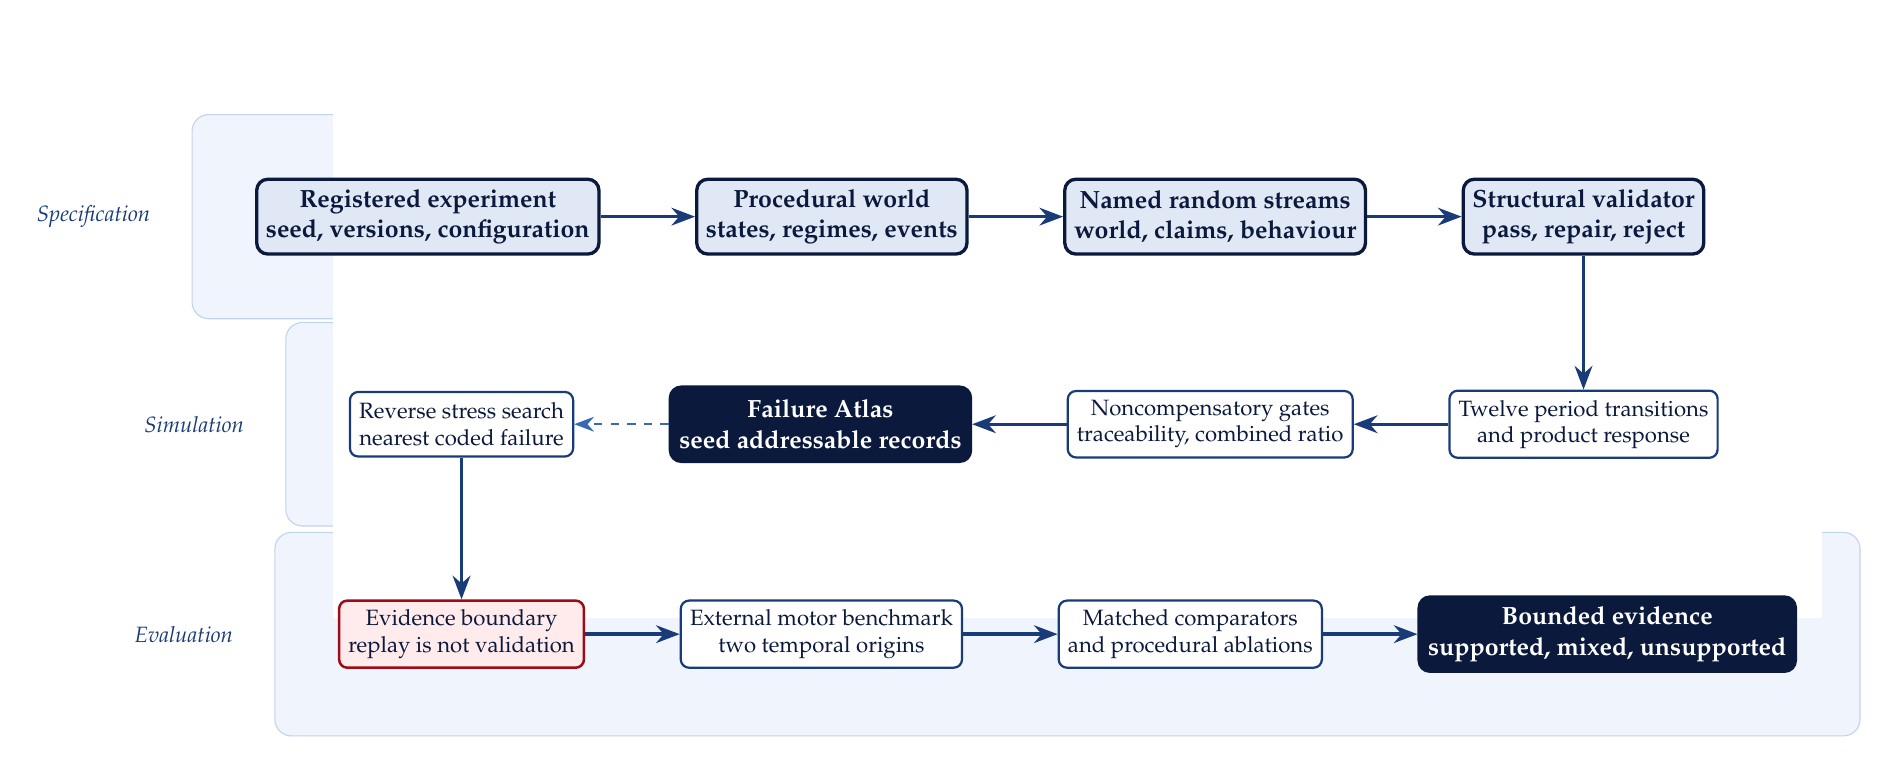
\begin{tikzpicture}[scale=1.0,node distance=9mm and 12mm]
  \path[fill=white] (-1.2,-5.1) rectangle (17.7,2.4);

  \node[primary] (register) {Registered experiment\\seed, versions, configuration};
  \node[primary,right=of register] (world) {Procedural world\\states, regimes, events};
  \node[primary,right=of world] (streams) {Named random streams\\world, claims, behaviour};
  \node[primary,right=of streams] (validator) {Structural validator\\pass, repair, reject};

  \node[secondary,below=17mm of validator] (transition) {Twelve period transitions\\and product response};
  \node[secondary,left=of transition] (gates) {Noncompensatory gates\\traceability, combined ratio};
  \node[terminal,left=of gates] (atlas) {Failure Atlas\\seed addressable records};
  \node[secondary,left=of atlas] (reverse) {Reverse stress search\\nearest coded failure};

  \node[alert,below=18mm of reverse] (boundary) {Evidence boundary\\replay is not validation};
  \node[secondary,right=of boundary] (empirical) {External motor benchmark\\two temporal origins};
  \node[secondary,right=of empirical] (ablation) {Matched comparators\\and procedural ablations};
  \node[terminal,right=of ablation] (evidence) {Bounded evidence\\supported, mixed, unsupported};

  \path (register) edge[mainflow] (world);
  \path (world) edge[mainflow] (streams);
  \path (streams) edge[mainflow] (validator);
  \path (validator) edge[mainflow] (transition);
  \path (transition) edge[mainflow] (gates);
  \path (gates) edge[mainflow] (atlas);
  \path (atlas) edge[feedback] (reverse);
  \path (reverse) edge[mainflow] (boundary);
  \path (empirical) edge[mainflow] (ablation);
  \path (ablation) edge[mainflow] (evidence);
  \path (boundary) edge[mainflow] (empirical);

  \begin{scope}[on background layer]
    \node[fill=navyfrost,draw=navyrule!35,rounded corners=6pt,
      fit=(register)(world)(streams)(validator),inner sep=8mm] (layer1) {};
    \node[fill=navyfrost,draw=navyrule!35,rounded corners=6pt,
      fit=(reverse)(transition)(gates)(atlas),inner sep=8mm] (layer2) {};
    \node[fill=navyfrost,draw=navyrule!35,rounded corners=6pt,
      fit=(boundary)(empirical)(ablation)(evidence),inner sep=8mm] (layer3) {};
  \end{scope}

  \node[layerlabel,left=4mm of layer1.west] {Specification};
  \node[layerlabel,left=4mm of layer2.west] {Simulation};
  \node[layerlabel,left=4mm of layer3.west] {Evaluation};
\end{tikzpicture}
\end{document}
